\chapter{Observations}


% Include the table
\begin{table*}
\caption{Summary of observations used to derive stellar atmospheric and orbital solutions for 5 EBLMs observed from the ground. The square brackets indicate the filter corresponding to the preceding number of observations.}              % title of Table
\label{Observeration_table_ground}      % is used to refer this table in the text
\centering                                    % used for centering table
\begin{tabular}{c l l  l l l l l l l l l l l l l }          % centered columns (4 columns)

\hline
\hline
 & J2349$-$32 & J2308$-$46 & J0218$-$31 & J1847$+$39 & J1436$-$13 \\
\hline
J2000.0 \\
$\alpha$  & $23^{\rm h}49^{'}15.23^{"}$ & $23^{\rm h}08^{'}45.66^{"}$ & $02^{\rm h}18^{'}13.24^{"}$ & $18^{\rm h}47^{'}52.34^{"}$ & $14^{\rm h}36^{'}46.42^{"}$\\
$\delta$ & $-32^{\circ}46' 17.5^{"}$ & $-46^{\circ}06^{'}36.6^{"}$  & $-31^{\circ}05^{'}17.3^{"}$ & $+39^{\circ}58^{'}51^{"}$ & $-13^{\circ}32^{'}35.5^{"}$\\
Vmag & 11.53 & 11.36 & 9.96 & 11.73 & 12.48\\
\\
$observations$ \\
WASP  & 8144 & 14,369 & 7872 & 9639 & 53,259 \\
SAAO 1-m  & 345 [I] & 474 [R]  & - & -  & 136 [R]\\
CTIO & - & - & 78 [g'] &- &- \\
& & & 62 [z'] \\
& & & 71 [r'] \\
& & & 70 [z'] \\
HAO  & - & - & - & 605 [CBB] & - \\
& & & & 311 [g'] \\
& & & & 371 [z'] \\
CORALIE & 20 & 19 & 70 & -& 20\\
INT & - & - & - &10 &-\\
\\
$Gaia$ \\
$G$
& $11.448 \pm 0.001$
& $11.381 \pm 0.001$
& $ 9.775 \pm 0.001$
& $11.755 \pm 0.001$
& $12.334 \pm 0.001$\\

$G_{BP} - G_{RP}$
& 0.7209
& 0.7276
& 0.7792
& 0.8177
& 0.7586 \\

parallax [mas]
& $3.851 \pm 0.042$ 
& $2.269 \pm 0.078$
& $3.844 \pm 0.042$
& $3.665 \pm 0.025$ 
& $2.145 \pm 0.051$\\\\

$photometry$ \\
APASS9 [B]  & 
$12.142 \pm 0.039$ &
$12.072 \pm 0.015$ &
$10.519 \pm 0.037$ &
$12.382 \pm 0.021$ &
$12.986 \pm 0.009$ \\

APASS9 [V]  & 
$11.541 \pm 0.010$ &
$11.517 \pm 0.045$ &
$9.903 \pm 0.026$ &
$11.913 \pm 0.022$ &
$12.480 \pm 0.014$ \\

APASS9 [g'] & 
$11.785 \pm 0.013$ &
$11.749 \pm 0.016$ &
$10.202 \pm 0.032$ &
$12.007 \pm 0.031$ &
$12.690 \pm 0.018$ \\

APASS9 [r'] & 
$11.438 \pm 0.033$ &
$11.382 \pm 0.014$ &
$9.779 \pm 0.029$ &
$11.704 \pm 0.006$ &
$12.354 \pm 0.021$ \\

APASS9 [i'] &
$11.317 \pm 0.013$ &
$11.286 \pm 0.006$ &
$9.632 \pm 0.079$ &
$11.548 \pm 0.006$ &
$12.231 \pm 0.064$ \\


TYCHO [B$_{\rm T}$] & 
$12.278 \pm 0.138$ &
$11.801 \pm 0.091$ &
$10.655 \pm 0.039$ &
$12.146 \pm 0.137$ &
- \\

TYCHO [V$_{\rm T}$] & 
$11.593 \pm 0.100$ &
$11.398 \pm 0.108$ &
$9.958 \pm 0.033$ &
$11.766 \pm 0.150$ &
- \\
2MASS [J] & 
$10.530 \pm 0.023$ &
$10.477 \pm 0.022$ &
$8.783 \pm 0.034$ &
$10.682 \pm 0.026$ &
$11.353 \pm 0.027$ \\

2MASS [H] & 
$10.249 \pm 0.022$ &
$10.270 \pm 0.024$ &
$8.555 \pm 0.031$ &
$10.362 \pm 0.032$ &
$11.040 \pm 0.021$ \\

2MASS [K$_{\rm S}$] & 
$10.184 \pm 0.019$ &
$10.166 \pm 0.020$ &
$8.493 \pm 0.025$ &
$10.306 \pm 0.021$ &
$10.987 \pm 0.019$ \\

DENIS [I$_{\rm C}$] & -  & - & - & - & $11.790 \pm 0.030$ \\
DENIS [J] & -  & - & - & - & $11.371 \pm 0.070$ \\
DENIS [K$_{\rm S}$] & -  & - & - & - & $10.912 \pm 0.070$ \\

E(B-V) & 
$0.010 \pm 0.034$ &
$0.007 \pm 0.034$ &
$0.024 \pm 0.030$ &
$0.088 \pm 0.030$ &
$0.072 \pm 0.034$ \\


\end{tabular}
\end{table*}








\begin{table*}
\caption{Summary of observations used to derive stellar atmospheric and orbital solutions for 5 EBLMs observed with K2. The square brackets indicate the filter corresponding to the preceding number of observations. }              % title of Table
\label{Observeration_table_K2}      % is used to refer this table in the text
\centering                                    % used for centering table
\begin{tabular}{c l l  l l l l l l l l l l l l l }  

\hline\hline                        % inserts double horizontal lines
 
 & J0055$+$00 
 & J0457$+$14 
 & J1652$-$19
 & J2217$-$04 \\
 
  
 & \object{EPIC220196587} 
 & \object{EPIC246712205}
 & \object{EPIC205148699}
 & \object{EPIC206500801}\\
 
\hline 
J2000.0 \\

$\alpha$  
& $00^{\rm h}55^{'}13.72^{"}$ 
& $04^{\rm h}57^{'}20.84^{"}$ 
& $16^{\rm h}52^{'}38.52^{"}$ 
& $22^{\rm h}17^{'}58.13^{"}$ \\


$\delta$ 
& $-00^{\circ}07' 54.00^{"}$
& $+14^{\circ}43' 30.40^{"}$
& $-19^{\circ}09' 41.70^{"}$
& $-04^{\circ}51' 52.60^{"}$\\

Vmag 
& 10.96 
& 12.14
& 12.75
& 12.18\\ \\

CORALIE
& 24
& 15
& 14
& 13\\ \\

$K2$ \\
Campaign 
& 8
& 13
& 2
& 3\\

data points 
& 3595
& 3703
& 2601
& 3199\\

Usable transits 
& 7
& 23
& 9
& 9\\ \\

$Gaia$ \\
$G$-mag
& $10.912 \pm 0.001$
& $11.916 \pm 0.001$
& $12.413 \pm 0.001$
& $12.003 \pm 0.001$ \\

$G_{BP} - G_{RP}$
& 0.8342
& 0.8439
& 1.0134
& 1.0294 \\

Parallax [mas]
& $3.158 \pm 0.062$ 
& $1.419 \pm 0.039$
& $2.081 \pm 0.113$
& $2.480 \pm 0.099$ \\ \\

$photometry$ \\
APASS9 [B]   
& $11.711 \pm 0.027$
& $12.677 \pm 0.036$
& $13.344 \pm 0.026$
& $13.047 \pm 0.053$ \\

APASS9 [V]  
& $11.043 \pm 0.032$
& $12.088 \pm 0.034$
& $12.614 \pm 0.043$
& $12.221 \pm 0.030$ \\

APASS9 [g']  
& $11.339 \pm 0.021$
& $12.374 \pm 0.035$
& $12.949 \pm 0.031$
& $12.582 \pm 0.040$ \\

APASS9 [r'] 
& $10.884 \pm 0.033$
& $11.920 \pm 0.021$
& $12.391 \pm 0.047$
& $11.957 \pm 0.024$ \\

APASS9 [i'] 
& $10.745 \pm 0.059$
& $11.772 \pm 0.072$
& $12.113 \pm 0.065$
& $11.922 \pm 0.215$ \\

2MASS [J] 
& $9.899 \pm 0.023$
& $10.801 \pm 0.023$
& $11.027 \pm 0.023$
& $10.749 \pm 0.022$ \\

2MASS [H] 
& $9.613 \pm 0.027$
& $10.663 \pm 0.032$
& $10.649 \pm 0.025$
& $10.404 \pm 0.022$ \\

2MASS [K$_{\rm S}$] 
& $9.534 \pm 0.021$
& $10.529 \pm 0.021$
& $10.554 \pm 0.022$
& $10.296 \pm 0.023$ \\

E(B-V)
& $0.023 \pm 0.034$
& $0.350 \pm 0.034$
& $0.298 \pm 0.034$
& $0.09 \pm 0.034$ \\

\hline


\end{tabular}
\end{table*}


Measuring the masses and radii of EBLM systems requires two types of data. The first type are spectroscopic observations which are taken at different phases of an EBLMs orbit. Spectra have two uses in this work: 1) they provide radial velocity measurements and 2) they can be co-added to estimate atmospheric parameters. I also use photometric colours to fit the spectral energy distribution to measure the photometric temperature and reddening. The second data type is transit photometry which sets the scale of each component. The quality of WASP photometry is not good enough to measure masses and radii to the desired precision of a few percent. To this end, I obtained higher-quality follow-up photometry which was used to determine the orbital solution. In the following sections I detail the origin and processing of data used in this work; this is summarised in Table \ref{Observeration_table_ground} \& \ref{Observeration_table_K2}. 



\section{Photometric colours}

Photometry for each target was extracted from the following catalogues: B$_{\rm T}$ and V$_{\rm T}$ magnitudes from the Tycho-2 catalogue \citep{2000A26A...355L..27H}; B, V, g$^{\prime}$, r$^{\prime}$ and i$^{\prime}$ magnitudes from data release 9 of the AAVSO Photometric All Sky Survey (APASS9; \citealt{2016yCat.2336....0H}; J, H and K$_{\rm s}$ magnitudes from the Two-Micron All-Sky Survey (2MASS; \citealt{2006AJ....131.1163S}; i$^{\prime}$, J and K magnitudes from the DEep Near-Infrared Southern Sky Survey (DENIS; \citealt{1997Msngr..87...27E}). The reddening maps by \citet{2011ApJ...737..103S} were used to estimate the total line-of-sight extinction in the direction of each target, ${\rm E}({\rm B}-{\rm V})$. Values of ${\rm E}({\rm B}-{\rm V})$ were calculated using the NASA/IPAC Extragalactic Database (NED) operated by the Jet Propulsion Laboratory, California Institute of Technology\footnote{https://ned.ipac.caltech.edu/help/extinction\_law\_calc.html}. Not all EBLMs have photometry in all catalogues; those that do are reported in Tables \ref{Observeration_table_ground} \& \ref{Observeration_table_K2}.

\section{Gaia}

\begin{figure}
    \centering
    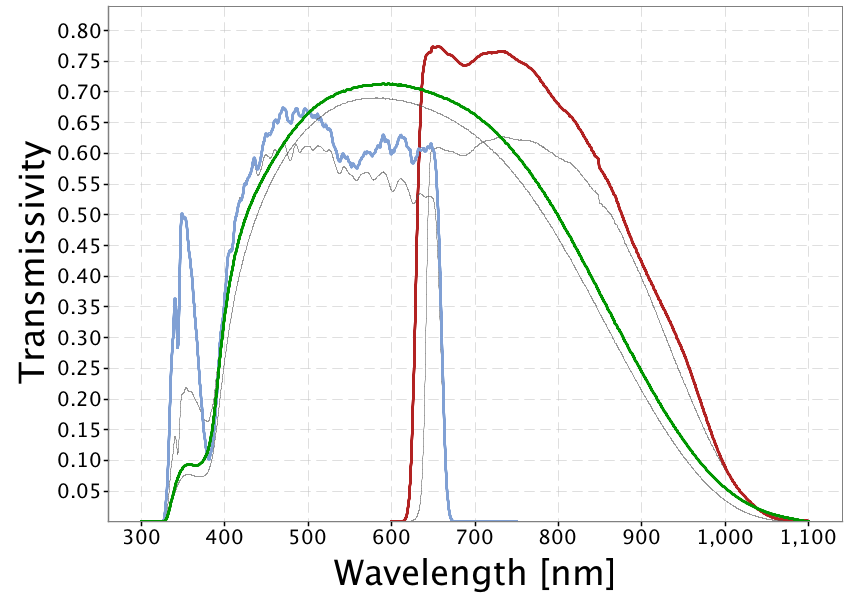
\includegraphics[scale=0.5]{6-images/GaiaDR2Passbands.png}
    \caption{The coloured lines in the figure show the revised passbands for $G$, $G_{\rm BP}$ and $G_{\rm RP}$ (green: $G$; blue: $G_{\rm BP}$; red: $G_{\rm RP}$), defining the Gaia DR2 photometric system. The thin, grey lines show the nominal, pre-launch passbands published in Jordi et al. 2010, used for Gaia DR1. Image taken from \textit{www.cosmos.esa.int}.}
    \label{methods:fig:gaia_EBLMs_passband}
\end{figure}


\begin{figure}
    \centering
    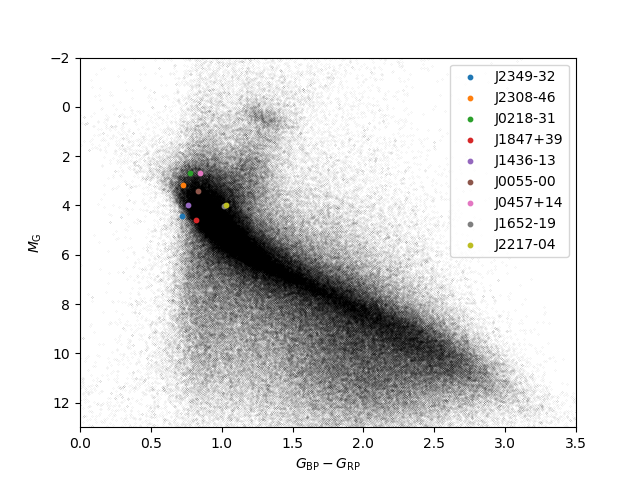
\includegraphics{6-images/Gaia_EBLMs.png}
    \caption{The $M_{\rm G}$-$G_{\rm BP}-G_{\rm RP}$ plane for 100 randomly selected source fields (black). The EBLMs used in the work are marked in red. }
    \label{methods:fig:gaia_EBLMsmy_label}
\end{figure}

% look here
% https://www.cosmos.esa.int/documents/29201/1770596/Lindegren_GaiaDR2_Astrometry_extended.pdf/1ebddb25-f010-6437-cb14-0e360e2d9f09
% Expand this section
% re- plot G Mag e.t.c

The second Gaia data release (Gaia DR2; \citealt{2018A&A...616A..10G}) provides mean flux counts in three bands -- $G$, $G_{\rm BP}$ and $G_{\rm RP}$ (see Fig. \ref{methods:fig:gaia_EBLMs_passband}). The $G$-band has a wider wavelength coverage and is optimised to determine astrometric solutions. The mean magnitudes $G_{\rm BP}$ and $G_{\rm RP}$ provide a ``slice'' through the spectral energy distribution of stars and reveal how red or blue a star is. I obtained the mean $G$, $G_{\rm BP}$ and $G_{\rm RP}$ magnitudes along with parralax measurements for all nine EBLM systems from Gaia DR2 using the Gaia archive\footnote{https://gea.esac.esa.int/archive} (Tables \ref{Observeration_table_ground} \& \ref{Observeration_table_K2}). There is evidence of systematic offsets in parallax measurements from Gaia DR2 (e.g. \citealt{2018ApJ...862...61S}) which is likely correlated with on-sky positions ($\alpha$ \& $\delta$), $G$ and $G_{\rm BP}$ - $G_{\rm RP}$ \citep{2018A&A...616A...2L}. Because the masses, radii and age of M-dwarfs in EBLMs in work do not depend on these results, I did not apply corrections to the parallax. The parallaxes and mean magnitudes are only used to briefly discuss tertiary components and volume-limited samples. I plot the position of all EBLMs in the $M_{\rm G}$-$G_{\rm BP}-G_{\rm RP}$ plane using data from 100 randomly selected source fields (Fig. \ref{methods:fig:gaia_EBLMsmy_label}). 

\section{Photometry: WASP}\label{WASP}

The WASP survey \citep{PollaccoSkillenCollierCameronEtAl2006} operates two survey instruments: one at the South African Astronomical Observatory (SAAO), South Africa, and another at the Observatorio del Roque de los Muchachos, La Palma.  Each instrument consists of an equatorial fork mount with eight cameras with 200-mm lenses and 2k$\times$2k CCD detectors. Each camera coveres approximately 64 square degrees per exposure. The data are processed by a detrending algorithm which was developed from the \textsc{SysRem} algorithm of \citet{2005MNRAS.356.1466T} and that is described by \citet{2007MNRAS.375..951C}. In July 2012, lenses on the southern installation (WASP-South) were changed to 85-mm with f/1.2 to search for brighter exoplanet hosts \citep{Smith2014}. Data from 85-mm lenses were not used in this study.

Photometry from the WASP cameras can suffer from a large amount of scatter due to clouds, instrumental artefacts, scattered light and other non-optimal observing conditions. I cleaned the data by removing points that were not detrended in the standard WASP reduction pipeline and removed points more than 0.5\,mag from the median magnitude of each star. Additional cleaning of the light curve was done by comparing each night of data to a phase-folded light curve binned into 500 phase bins. Any measurement $3$-$ \sigma$ or more from the mean in each bin was excluded. The entire night of data was excluded if more than a quarter of the night's data was excluded this way or if there are fewer than 10 observations. The binned light curve is then inspected by eye to further exclude bad data points.

\section{Photometry: SAAO 1-m}

The SAAO hosts an equatorial-mounted 1-m telescope built by Grubb and Parsons that is equipped with an STE4 CCD camera with 1024\,$\times$\,1024 pixels. This camera was operated in $2 \times 2$ binning mode to reduce readout time. I observed a single transit for J2349$-$32 on 18 October 2016 and J2308$-$46 on  12 October 2016 using $I$ (exposure time of $t_{\rm exp}$ = 50\,s) and $R$ ($t_{\rm exp}$ = 40\,s) Bessel filters. Jess Kirkby-kent observed J1436$-$13 on 23 April 2017 in the $R$ ($t_{\rm exp}$ = 40\,s) Bessel filter. Photometry was extracted using standard aperture photometry routines \citep{Southworth2009} and uncertainties were estimated from photon counting statistics. A by-eye approach was used to clean the light curve and select the best comparison star in the $5' \times 5'$ field. A slow variation in differential magnitude with time was observed corresponding to changes in the effective airmass. To correct for this, I defined out-of-transit regions and then used the IDL/AMOEBA\footnote{http://www.harrisgeospatial.com/docs/AMOEBA.html} routine to fit a polynomial which minimised the square of the magnitude residuals. I then divided this trend resulting in light curves which were normalised to zero differential magnitude.  


\section{Photometry: HAO}

\begin{figure}[htb]

  \centering
  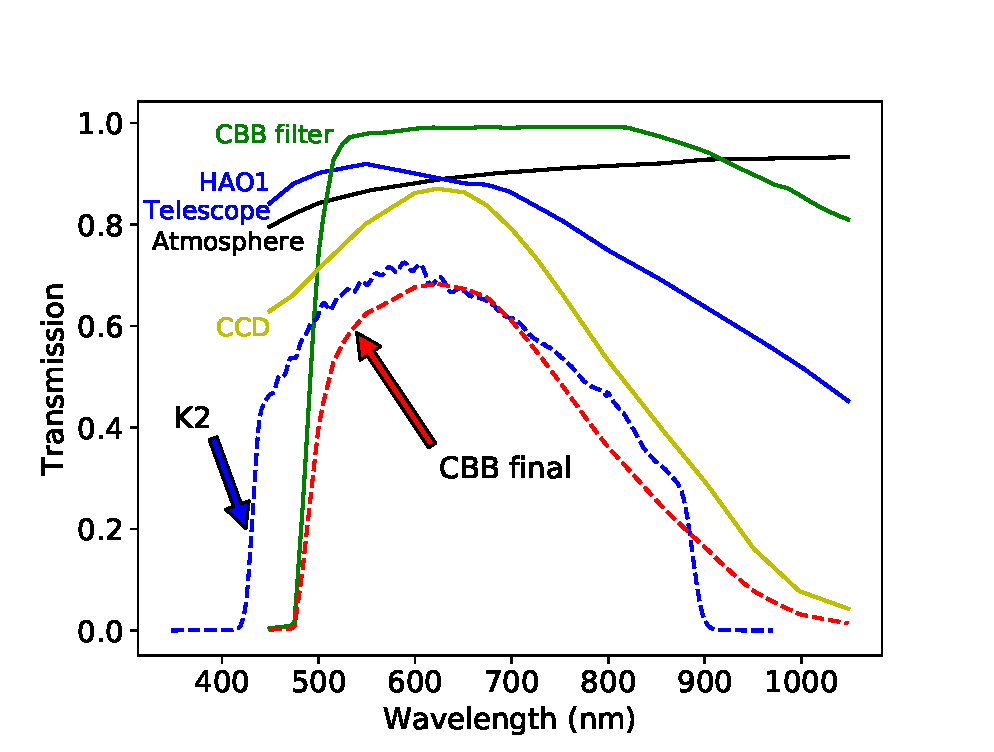
\includegraphics{6-images/CBB_response.eps}
  \caption{The response function of the HAO+CBB instrument. The atmospheric transmission is plotted in black, the transmission of the HAO telescope in blue-solid, the CBB filter in green and CCD response in yellow. The final response of HAO-1 with the CBB filter is plotted in red-dashed along with the K2 transmission (blue-dashed). The atmospheric transmission line originated from equations for Rayleigh, aerosol and ozone extinction vs. wavelength for Palomar Observatory \protect\citep{1975ApJ...197..593H}. Coefficients were adjusted until they agreed with observations of extinction at HAO over a few dates.}
  \label{HAO_CBB}
\end{figure}


\begin{figure}[htb]
  \centering
  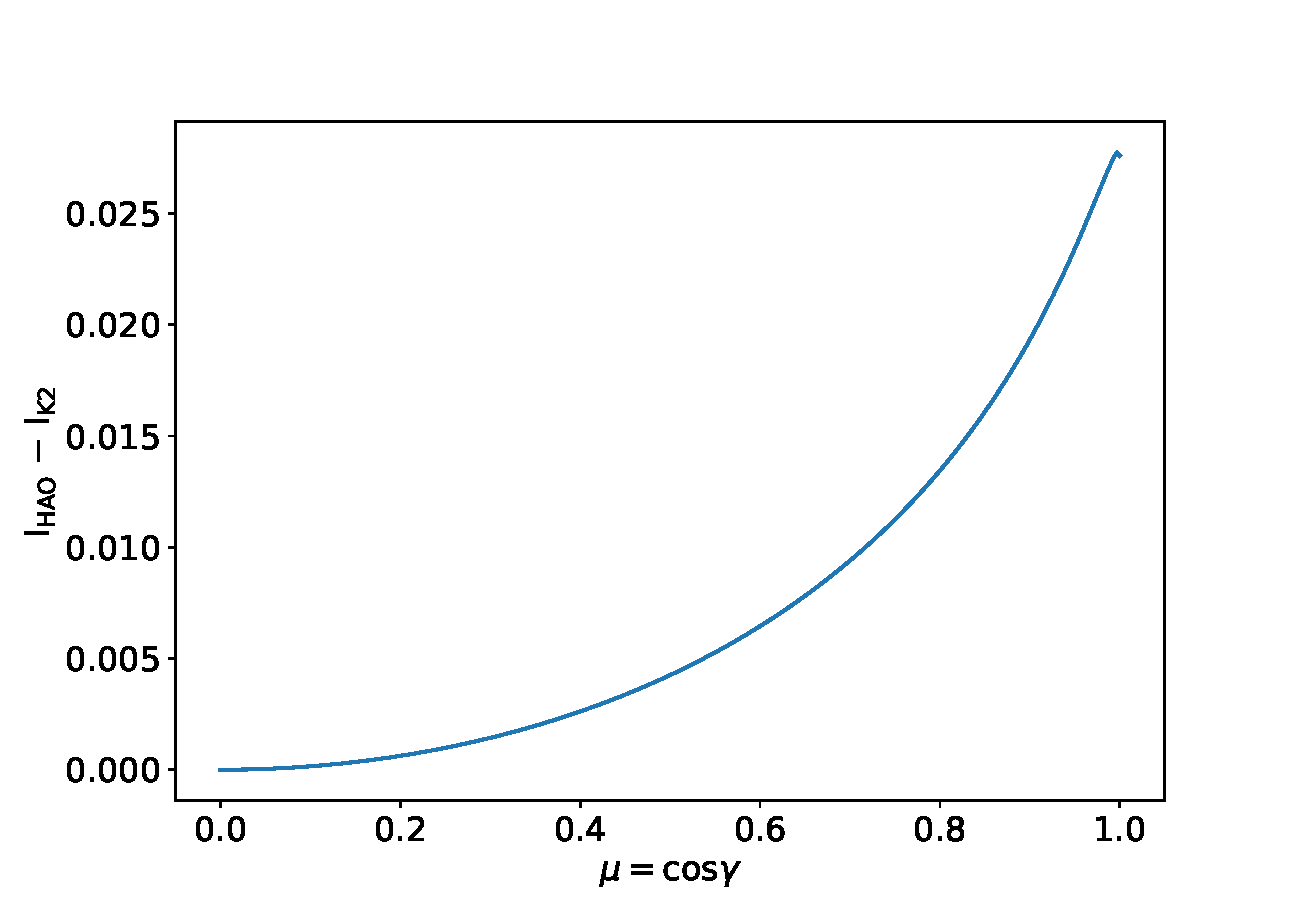
\includegraphics[scale=0.8]{6-images/kepVShao.eps}
  \caption{The difference in theoretical intensity acoss the stellar disk for the HAO+CBB filter and the Kepler/K2 Filter as a function of the angle between a line normal to the stellar surface and the line of sight of the observer ($\gamma$) for J1847$+$39. }
  \label{kepVShao}
\end{figure}

Optical photometry for J1847$+$39 was provided by Bruce Gary at the Hereford Arizona Observatory (HAO). Three separate transits were observed with a Meade 14-inch LX200GPS telescope. The first was obtained with the clear blue-blocking filter (CBB) on 9 October 2009 with $t_{\rm exp} = 100$\,s. The second was with a $g'$ filter on 18 May 2011 with $t_{\rm exp} = 60$\, s. The last was with a $z'$ filter on 15 June 2010 with $t_{\rm exp} = 60$\, s. Aperture photometry was extracted using standard photometry routines with systematic trends removed and outliers rejected.  I used transmission information of the telescope throughput, atmosphere, filter and CCD\footnote{http://www.brucegary.net/HAO/} to calculate the final transmission of HAO with the CBB filter (see Fig.~\ref{HAO_CBB}). I used the four-parameter limb-darkening look-up table for the K2 passband instead of the CBB filter due to the similarity in final transmission since I do not have access to a four-parameter look-up table for the CBB filter. In Sect.~\ref{limb_darkening_section} I fit light curves
using the two-parameter quadratic limb-darkening instead of the Claret law. The final response function in Fig.~\ref{HAO_CBB} is used  along with estimates of stellar atmospheric parameters (from Sect. \ref{methods:SED} \& \ref{methods:atmospheric_parameters}) to calculate quadratic coefficients using \textsc{ldtk} \citep{Parviainen2015}. 

The discrepancy between the K2 and HAO+CBB pass-band differ in the blue where the limb-darkening is most significant. I assessed this by using \textsc{ldtk} to synthesise intensity profiles for J1847$+$39 across the stellar disk for each pass-band and calculate the discrepancy as a function of $\gamma$ (the angle between a line normal to the stellar surface and the line of sight of the observer; Fig. \ref{kepVShao}). The K2 pass-band emits 2.5\,\% less flux than what would be observed with HA0+CBB towards the limb. I calculated quadratic limb-darkening coefficients for the K2 pass-band to be $u_1 = 0.496 \pm 0.050$, $u_2 = 0.157 \pm 0.050$ and for the HAO+CBB pass-band to be $u_1 = 0.468 \pm 0.050$, $u_2 = 0.148 \pm 0.051$. These are comparable within 1-$\sigma$ and so adopting the K2 pass-band for J1847$+$39 will have a negligible effect on the transit shape.


\subsection{Photometry: CTIO}

J0218-31 was observed on 14 November 2010 with the CTIO-0.9-m telescope and Tek2K CCD camera. The detector consists of a 2K$\times$2K array of $15\mu m$ pixels placed at Cassegrain focus giving a $0.4^{\prime\prime}$/pixel plate scale. Thus the entire array projects to a $13.7^{\prime}$ FOV.   The observed signal is fed into four amplifiers causing the raw images to have a quadrant effect with the readnoise between 3.9-4.5~$e^{-}$ and gain of 2.5-2.8~$e^{-}$/ADU, depending on the amplifier. The detector has a readout time of 39 seconds and a 60,000 count well depth before non-linearity sets in $1\times 1$ binning mode.

J0218-31 and the surrounding field were monitored throughout the night using the Sloan $griz$ filter set alternating continuously between all four filters. Exposure times were chosen to maximise the flux in the target star and nearby reference stars while keeping the peak pixel value in J0218$-$31 below $60,000$ counts. The telescope was defocused to allow for longer exposure times to build up signal in the fainter reference stars without saturating J0218-31. They adopted an exposure time of 10~seconds for the $g^{\prime}$, $r^{\prime}$, and $i^{\prime}$--band observations and longer exposures of 15~seconds in the $z^{\prime}$ filter where the detector is less sensitive. An overall light curve cadence of approximately 3.3 minutes was achieved in each filter accounting for the exposure times,  the read out time, and filter changes. The light curves were created from approximately 75 images taken in each filter during the single observing night.

A set of 11 bias calibration frames and 11 dome flat fields in all four filters were  obtained at the beginning of the observing night. The images were processed in a standard way using routines written by L.\ Hebb in the IDL programming language.  Each of the four amplifiers was processed independently.  All object and calibration frames were first overscan corrected (by subtracting a line-by-line median overscan value), bias subtracted and then trimmed.  Stacked bias images were created by averaging all bias frames observed each night and subtracted from all science  and flat-field frames.  All dome flats were averaged into a single dome flat in each filter and then applied to the trimmed and bias-corrected science images. 

Source detection and aperture photometry were performed on all processed science images using the Cambridge Astronomical Survey Unit catalogue extraction software \citep{2001NewAR..45..105I}. The  software  has  been  compared  with  SExtractor \citep{1996A26AS..117..393B} and found to be very similar in the completeness, astrometry and photometry tests.\footnote{\url{https://www.ast.cam.ac.uk/ioa/research/vdfs/docs/reports/simul/index.html}} This photometry software was applied to all processed images of J0218-31.  Adopting conservative parameters to define the detection threshold, the target star and dozens of fainter stars in the field were detected in each image.  Aperture photometry was performed on all detected stars using a 5~pixel radius circular aperture, which was selected to match the typical seeing. Five bright, non-variable reference stars were selected from the many detected stars and used to perform differential photometry on the target star.  In each image, the flux from all reference stars was summed into a single \textit{super} comparison star that was divided by the aperture flux from J0218-31 and converted to a differential magnitude.

\section{Photometry: K2}

The Kepler mission was launched in 2009 and spent over four years monitoring over 150,000 stars in the constellations of Cygnus and Lyra\footnote{https://keplerscience.arc.nasa.gov/objectives.html}. The spacecraft has a 0.95-m Schmidt telescope
with a 110-square degree field of view imager (pixel scale of 4"/ pixel). The primary science goal of Kepler was to detect and characterise terrestrial planets ($R_p < 2.5\,R_{\oplus}$) which reside in the habitable zone of Sun-like stars. Observations for tens of thousands of stars with short cadence (1-min) and many more thousands with long cadence (30-min) lead to the discovery of many exoplanet (e.g. \citealt{2013ApJ...768...14W}; \citealt{2012ApJ...747..144M}; \citealt{2013ApJ...777....3N}) and eclipsing binary systems (e.g. \citealt{2011Sci...331..562C}; \citealt{2011ApJS..197....4W}; \citealt{2011ApJ...736L...4S}). 

Kepler exceeded its nominal mission lifetime (3 years) by 1 year until the loss of the second of four reaction wheels in May 2013. In the following months the mission was rebranded "K2" - a name chosen to honour the two remaining reaction wheels or the second Kepler mission \citep{2014PASP..126..398H}. The K2 mission consists of sequential observing \textit{campaigns} in the ecliptic plane. This is so the torque excerpted on the spacecraft by solar wind pressure can be balanced with altitude thrusters and the two remaining reaction wheels to control pointing. The pointing is significantly worse than the original Kepler mission but the photometric quality approaches that of the original mission after decorrelation of the position-dependent instrument noise. Four EBLMs with spectroscopic orbits published by \citet{Triaud2017} have been observed with K2 (J0055$+$00, J0457$+$14,  J1652$-$19 and J2217$-$04). In the following sections I describe how  photometry was extracted from target pixel files and how I corrected for position-dependent instrumental noise.


\subsection{Extraction}\label{observations:K2:extract}

The target pixel files for each target were acquired from the Mikulski Archive for Space Telescopes (MAST\footnote{archive.stsci.edu}). I used data from Gaia DR2 to inform how masks were created for the target pixel files. For J0055$-$00, J0457$+$14 and J2217$-$04 I found no significant ($\Delta G < 6$) companions within 1' so I choose masks which match the shape of the stellar profile of the 100$^{th}$ target pixel file (Fig. \ref{observations:target_pixel_files}). For J1652$-$19 I found three close companions within 20" eastwards (Fig. \ref{observations:J1652}). The brightest ($\Delta G = 3.33$) is 14" away at a position angle (PA) of 107$^{\circ}$. This, and the other two fainter companions at PA = 85$^{\circ}$ ($\Delta G = 4.28$) and PA = 54$^{\circ}$ ($\Delta G = 4.17$) may be visible in the target pixel files. If I used full-frame photometry I could expect up to 9\% contamination. I excluded these stars by creating a box-like mask at the east and south side of J1652$-$19. The pointing precision (estimated from centroiding; Sect. \ref{observations:K2:detrending}) is above 1 pixel and so very little flux from the three nearby stars entered into the aperture. I used the \textsc{kepextract} function \citep{pyke3} to extract raw photometry using the masks created for each system. 

 \begin{figure*}
\centering
 \begin{subfigure}[b]{0.5\linewidth}
    \centering
    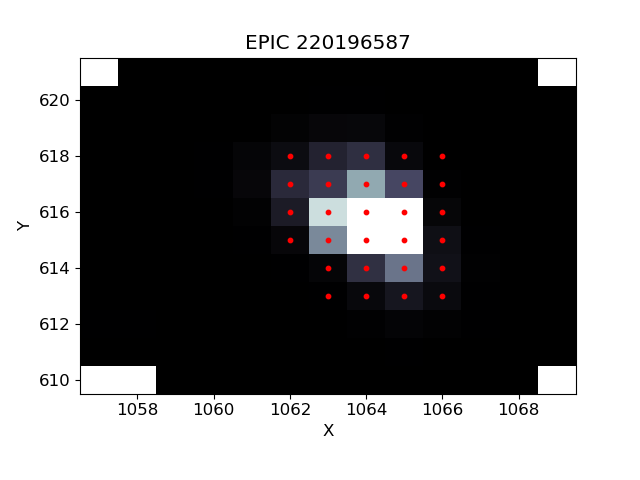
\includegraphics[width=\linewidth]{6-images/EPIC220196587_PIXEL_FILE.png} 
    %\caption{} 
    \label{EPIC220196587_PIXEL_FILE} 
    \vspace{4ex}
  \end{subfigure}%% 
  \begin{subfigure}[b]{0.5\linewidth}
    \centering
    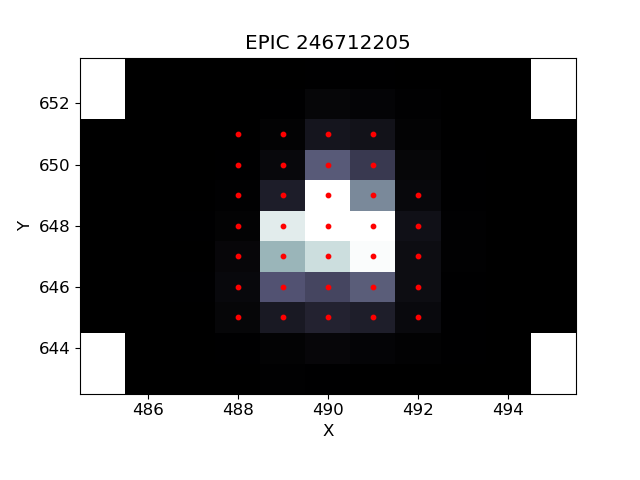
\includegraphics[width=\linewidth]{6-images/EPIC246712205_PIXEL_FILE.png} 
    %\caption{} 
    \label{EPIC246712205_PIXEL_FILE} 
    \vspace{4ex}
  \end{subfigure} 
  \begin{subfigure}[b]{0.5\linewidth}
    \centering
    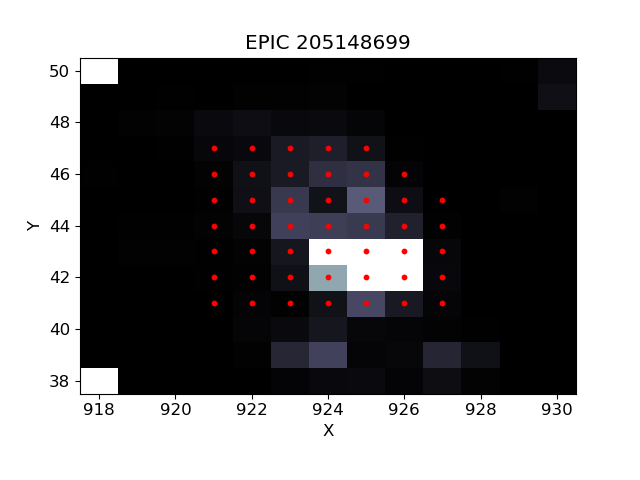
\includegraphics[width=\linewidth]{6-images/EPIC205148699_PIXEL_FILE.png} 
    %\caption{} 
    \label{EPIC205148699_PIXEL_FILE} 
  \end{subfigure}%%
  \begin{subfigure}[b]{0.5\linewidth}
    \centering
   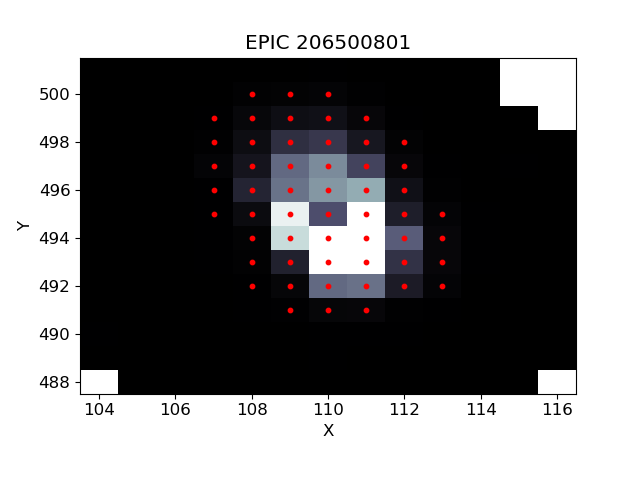
\includegraphics[width=\linewidth]{6-images/EPIC206500801_PIXEL_FILE.png}
    %\caption{} 
    \label{EPIC206500801_PIXEL_FILE} 
  \end{subfigure} 
  \caption{The 100$^{th}$ target pixel frame for all EBLM systems. Red dots indicate a pixel that was used to in the aperture photometry using \textsc{pyke}. }
  \label{observations:target_pixel_files}   
\end{figure*}


\begin{figure}
    \centering
    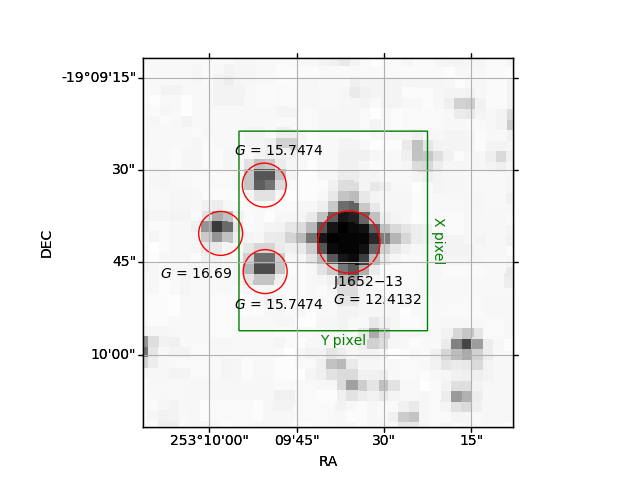
\includegraphics{6-images/J1652.png}
    \caption{The 2MASS finder image of J1652$-$19. Red apertures mark significant stars in the field with Gaia magnitudes labelled. The green box approximates the extent of the K2 pixel files for J1652$-$19 (Fig. \ref{observations:target_pixel_files}).}
    \label{observations:J1652}
\end{figure}




\subsection{De-trending}\label{observations:K2:detrending}

The \textsc{kepextract} function fitted a 2-dimensional Gaussian to the target pixel files in each frame to measure each stars CCD position as a function of time. I used the \textsc{k2sc} algorithm \citep{2016MNRAS.459.2408A} to detrend against time, x-position and y-position using Gaussian processes. I used an exponential-squared kernel provided by the \textsc{george} with the \textsc{detrender} function \citep{hodlr} provided with \textsc{k2sc}. This was used to predict variations in the out-of-transit photometry correlated with time and pixel positions. The remaining outliers between transits were detected using basic iterative sigma-clipping, where a data point was excluded if the flux value was over 5-$\sigma$ from median out-of-eclipse flux level. Although I observed significant "jumps" in photometry continuum levels and evolving noise profiles, I assumed that the remaining variation is caused by stellar activity/binary interaction.

		


\section{Spectroscopy: CORALIE}

CORALIE is a fiber-fed \'{e}chelle spectrograph installed on the 1.2-m Leonard Euler telescope at the ESO La Silla Observatory and has a resolving power R = 50,000\,--\,60,000 \citep{2001A&A...379..279Q,Wilson2008}. The spectra used in this study were all obtained with an exposure time $t_{\rm exp} = 600$\,s. Observations of J0218$-$31 include spectra obtained through the transit that show the Rossiter-McLaughlin effect. The spectra for each star were processed with the CORALIE standard reduction pipeline \citep{26AS..119..373B}. Radial velocity measurements were obtained using standard cross-correlation techniques (using numerical masks) and checked for obvious outliers \citep{Triaud2017}. Each spectrum was corrected into the laboratory reference frame and co-added onto a common wavelength range. Maximum and median filters were applied to identify continuum regions which were fitted with spline functions (one every nm) to normalise the spectra (a standard function within \textsc{ispec} v20161118; \citealt{Blanco-Cuaresma2017}). 


\section{Spectroscopy: INT}

Spectra for J1847$+$39 were obtained using the intermediate dispersion spectrograph (IDS) mounted on the 2.5-m Isaac Newton telescope (INT) at the Roque de Los Muchachos Observatory. The 235-mm camera and EEV10 CCD detector was used with the H1800V grating to obtain spectra in a small region around the H$\alpha$ line with R$\approx$10,000\footnote{Calculated from http://www.ing.iac.es/}. A total of 10 spectra were obtained for J1847$+$39 with an exposure time $t_{\rm exp} = 600$-$900$\, s. Radial velocity measurements were extracted using cross-correlation routines provided within \textsc{ispec}. I used a synthetic F0 spectrum as a template with a mask applied to the core of the H$\alpha$ line. A Gaussian function was fitted to the peak in each cross-correlation function to obtain the radial velocity measurement (the peak of the Gaussian function), and uncertainty (standard deviation of the Gaussian function). Each spectrum was corrected into a laboratory reference frame and co-added onto a common wavelength range. The relatively small wavelength range does not permit the use of maximum and median filters to normalise the spectra. I instead identified suitable continuum regions by-eye and normalised the spectrum using a second-order polynomial fit by least-squares.  

\section{Lucky imaging}

The lucky-imaging technique (e.g. \citealt{2006A&A...446..739L}) was used to obtain high-resolution images of J2308$-$46, J2349$-$32, J0055-00, J1652-19 and J2217-04 in July 2017, in order to search for stars contributing contaminating light, as well as potential bound companions to the eclipsing binaries. The observations were conducted using the Two Colour Instrument (TCI) on the Danish 1.54-m Telescope at La Silla Observatory. The TCI consists of two Electron Multiplying CCDs capable of imaging simultaneously in two passbands at a frame rate of $10$\,Hz, with a $40"\times40$" field of view. The `red' arm has a passband similar to a combined $i+z$ filter or the Cousins $I$ filter, whilst the `visible' arm has a mean wavelength close to that of the Johnson $V$ filter. A detailed description of the instrument  can be found in \citet{2015A26A...574A..54S} and  the lucky imaging reduction pipeline is described by \citet{2012A&A...542A..23H}.

The observations and data reduction were carried out using the method outlined in \citet{2018A26A...610A..20E}, and is briefly described here. Both targets were observed for 170\,s. The raw data were reduced automatically by the instrument pipeline, which performs bias and flat frame corrections, removes cosmic rays, and determines the quality of each frame, with the end product being ten sets of stacked frames, ordered by quality. The data were run through a custom star-detection algorithm that is described in \citet{2018A26A...610A..20E}, which is designed to detect close companion stars that may not be fully resolved.